\documentclass{article}
\usepackage{ctex}
\usepackage{amsmath}
\usepackage{geometry}
\usepackage{graphicx}
\usepackage{float} 
\usepackage{tikz}
\usetikzlibrary{calc}
\usetikzlibrary{positioning}
\usetikzlibrary{graphs,graphs.standard}
\graphicspath{{figure/}}
\geometry{a4paper,left=2cm,right=2cm,top=2cm}
\title{Discrete Mathematics Quiz 4\\\small{2021 - 2022 \enspace 春夏学期 \enspace 郑文庭班}}
\author{Shd0wash}
\date{\today}
\setlength{\parskip}{1em}
\setlength{\baselineskip}{20pt}
\setlength{\parindent}{0em}
\begin{document}

\maketitle

1. Suppose we are trying to write down, in predicate logic, a theory explaining the success of failure of various historical leader. We have two predicates 
taller$(x,y)$(``$x$ was taller than $y$'') and successful($x$)(``$x$ was successful as a leader''), as well as the usual tools of predicate logic and can refer to 
the specific leaders by name. Express each of the following statements in mathematical form. Note that statements are not connected, and no guarantees are 
made about whether any of them are actually true. (18\%)\\
(a) Lincoln was the tallest leader.\\
(b) Napoleon was at least as tall as any unsuccessful leader.\\
(c) No two leaders had the same height.

2. A 4-digit number is called a palindrome if it is the same when the digits are read in reverse. For example, 7337 and 3333 are 4-digit palindromes, but 1337 
and 0990 are not. Note that 0990 does not count because it is actually a 3-digit number. A 4-digit number is called an almost-palindrome if there is a way to 
exchange exactly one digit so that the result is a 4-digit palindrome. For example, 1337, 1501 and 1990 are 4-digit almost-palindromes(they could become 1331 
or 7337, 1001 or 1551, and 1991), but 1234, 0991 and 1331 are not. The issue with 0991 is again that it is actually a 3-digit number, and the issue with 1331 
is that if you change any digit, then it becomes a non-palindrome. How many 4-digit almost-palindromes are there? (12\%)

3. Suppose a recurrence relation has the form  $a_{n} = c_{1}a_{n-1} + c_{2}a_{n-2} + c_{3}$, $c_{1}, \enspace c_{2}, \enspace c_{3}$ are unknown variables, 
and $a_{0} = 0, \enspace a_{1} = 1, \enspace a_{2} = 4, \enspace a_{3} = 11 \enspace and \enspace a_{4} = 26$. Find the solution to this recurrence solution. 
(15\%)

\clearpage

4. The grid graph $G_{m,n}$ refers to the graph obtained by taking an $m \times n$ rectangular grid of streets $(m \leq n)$. For example:
\begin{figure}[htbp]
    \centering
    \begin{minipage}[t]{0.48\textwidth}
        \centering
        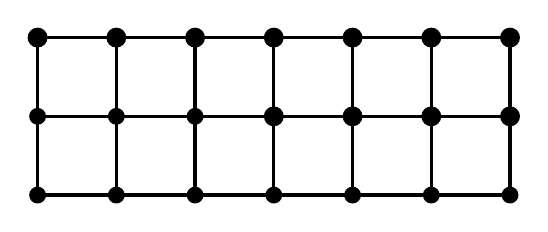
\begin{tikzpicture}
            \begin{scope}[every node/.style={thick, circle, draw, fill, scale = 0.3}]
                \node (0) at (0,0) {0};
                \node (1) at (1,0) {1};
                \node (2) at (2,0) {2};
                \node (3) at (3,0) {3};
                \node (4) at (4,0) {4};
                \node (5) at (5,0) {5};
                \node (6) at (6,0) {6};
                \node (7) at (0,1) {7};
                \node (8) at (1,1) {8};
                \node (9) at (2,1) {9};
                \node (10) at (3,1) {10};
                \node (11) at (4,1) {11};
                \node (12) at (5,1) {12};
                \node (13) at (6,1) {13};
                \node (14) at (0,2) {14};
                \node (15) at (1,2) {15};
                \node (16) at (2,2) {16};
                \node (17) at (3,2) {17};
                \node (18) at (4,2) {18};
                \node (19) at (5,2) {19};
                \node (20) at (6,2) {20};
            \end{scope}

            \begin{scope}[every edge/.style={draw=black, very thick}]
                \path [-] (0) edge (1);
                \path [-] (1) edge (2);
                \path [-] (2) edge (3);
                \path [-] (3) edge (4);
                \path [-] (4) edge (5);
                \path [-] (5) edge (6);
                \path [-] (7) edge (8);
                \path [-] (8) edge (9);
                \path [-] (9) edge (10);
                \path [-] (10) edge (11);
                \path [-] (11) edge (12);
                \path [-] (12) edge (13);
                \path [-] (14) edge (15);
                \path [-] (15) edge (16);
                \path [-] (16) edge (17);
                \path [-] (17) edge (18);
                \path [-] (18) edge (19);
                \path [-] (19) edge (20);
                \path [-] (0) edge (7);
                \path [-] (7) edge (14);
                \path [-] (1) edge (8);
                \path [-] (8) edge (15);
                \path [-] (2) edge (9);
                \path [-] (9) edge (16);
                \path [-] (3) edge (10);
                \path [-] (10) edge (17);
                \path [-] (4) edge (11);
                \path [-] (11) edge (18);
                \path [-] (5) edge (12);
                \path [-] (12) edge (19);
                \path [-] (6) edge (13);
                \path [-] (13) edge (20);
            \end{scope}
        \end{tikzpicture}
        \caption{$G_{2,6}$}
    \end{minipage}
    \begin{minipage}[t]{0.48\textwidth}
        \centering
        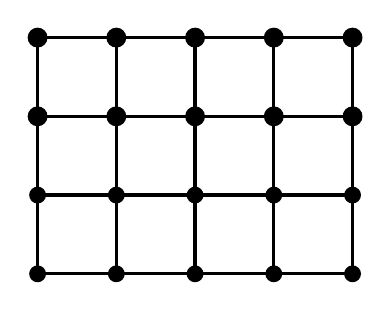
\begin{tikzpicture}
            \begin{scope}[every node/.style={thick, circle, draw, fill, scale = 0.3}]
                \node (0) at (0,0) {0};
                \node (1) at (1,0) {1};
                \node (2) at (2,0) {2};
                \node (3) at (3,0) {3};
                \node (4) at (4,0) {4};
                \node (5) at (0,1) {5};
                \node (6) at (1,1) {6};
                \node (7) at (2,1) {7};
                \node (8) at (3,1) {8};
                \node (9) at (4,1) {9};
                \node (10) at (0,2) {10};
                \node (11) at (1,2) {11};
                \node (12) at (2,2) {12};
                \node (13) at (3,2) {13};
                \node (14) at (4,2) {14};
                \node (15) at (0,3) {15};
                \node (16) at (1,3) {16};
                \node (17) at (2,3) {17};
                \node (18) at (3,3) {18};
                \node (19) at (4,3) {19};
            \end{scope}

            \begin{scope}[every edge/.style={draw=black, very thick}]
                \path [-] (0) edge (1);
                \path [-] (1) edge (2);
                \path [-] (2) edge (3);
                \path [-] (3) edge (4);
                \path [-] (5) edge (6);
                \path [-] (6) edge (7);
                \path [-] (7) edge (8);
                \path [-] (8) edge (9);
                \path [-] (10) edge (11);
                \path [-] (11) edge (12);
                \path [-] (12) edge (13);
                \path [-] (13) edge (14);
                \path [-] (15) edge (16);
                \path [-] (16) edge (17);
                \path [-] (17) edge (18);
                \path [-] (18) edge (19);
                \path [-] (0) edge (5);
                \path [-] (5) edge (10);
                \path [-] (10) edge (15);
                \path [-] (1) edge (6);
                \path [-] (6) edge (11);
                \path [-] (11) edge (16);
                \path [-] (2) edge (7);
                \path [-] (7) edge (12);
                \path [-] (12) edge (17);
                \path [-] (3) edge (8);
                \path [-] (8) edge (13);
                \path [-] (13) edge (18);
                \path [-] (4) edge (9);
                \path [-] (9) edge (14);
                \path [-] (14) edge (19);
            \end{scope}
        \end{tikzpicture}
        \caption{$G_{3,4}$}
    \end{minipage}
\end{figure}

(a) For which positive integers $m$ and $n$ does $G_{m,n}$ have an Euler circuit?\\
(b) For which positive integers $m$ and $n$ does $G_{m,n}$ have an Euler path but no Euler circuit?\\
(c) For which positive integers $m$ and $n$ does $G_{m,n}$ have a Hamilton circuit?\\
(d) For which positive integers $m$ and $n$ does $G_{m,n}$ have a Hamilton path but no Hamilton circuit?\\
(e) How many spanning trees does $G_{1,2}$ have? (25\%)

5. A regular polyhedron(正多面体) means that all faces of the polyhedron are congruent(相同的), and all polyhedral angles are congruent. For example:
\begin{figure}[htbp]
    \centering
    \begin{minipage}[t]{0.3\textwidth}
        \centering
        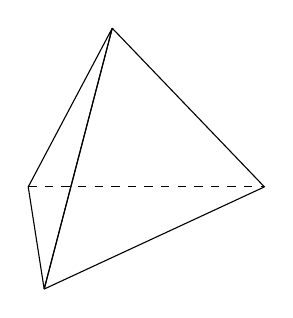
\begin{tikzpicture}[line join=bevel,x=1cm,y=1cm,z=-0.5cm]
            \coordinate (A1) at (0,0,0);
            \coordinate (A2) at (3,0,0);
            \coordinate (A3) at (1.5,0,2.595);
            \coordinate (B1) at (1.5,2.448,0.866);

            \draw [dashed] (A1) -- (A2);
            \draw [fill opacity=0.7] (A1) -- (A3) -- (B1) -- cycle;
            \draw [fill opacity=0.7] (A2) -- (A3) -- (B1) -- cycle;
        \end{tikzpicture}
        \caption{\textit{Tetrahedron}}
    \end{minipage}
    \begin{minipage}[t]{0.3\textwidth}
        \centering
        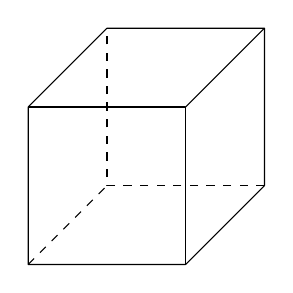
\begin{tikzpicture}[line join=bevel, z=-0.5cm]
            \coordinate (A1) at (0,0,0);
            \coordinate (A2) at (2,0,0);
            \coordinate (A3) at (2,2,0);
            \coordinate (A4) at (0,2,0);
            \coordinate (B1) at (0,0,2);
            \coordinate (B2) at (2,0,2);
            \coordinate (B3) at (2,2,2);
            \coordinate (B4) at (0,2,2);

            \draw [dashed] (A2) -- (A1) -- (A4);
            \draw [dashed] (B1) -- (A1);
            \draw [fill opacity=0.7] (A2) -- (A3) -- (A4) -- (B4) -- (B1) -- (B2) -- cycle;
            \draw [fill opacity=0.7] (B2) -- (B3) -- (B4);
            \draw [fill opacity=0.7] (B3) -- (A3);
        \end{tikzpicture}
        \caption{\textit{Cube}}
    \end{minipage}
    \begin{minipage}[t]{0.3\textwidth}
        \centering
        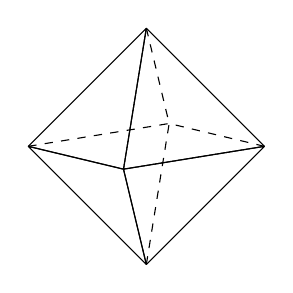
\begin{tikzpicture}[line join=bevel, z=-5.5]
            \coordinate (A1) at (0,0,-1.5);
            \coordinate (A2) at (-1.5,0,0);
            \coordinate (A3) at (0,0,1.5);
            \coordinate (A4) at (1.5,0,0);
            \coordinate (B1) at (0,1.5,0);
            \coordinate (C1) at (0,-1.5,0);

            \draw [dashed] (B1) -- (A1) -- (C1);
            \draw [dashed] (A2) -- (A1) -- (A4);
            \draw [fill opacity=0.7] (A2) -- (A3) -- (B1) -- cycle;
            \draw [fill opacity=0.7] (A2) -- (A3) -- (C1) -- cycle;
            \draw [fill opacity=0.7] (A4) -- (A3) -- (B1) -- cycle;
            \draw [fill opacity=0.7] (A4) -- (A3) -- (C1) -- cycle;
        \end{tikzpicture}
        \caption{\textit{Octahedron}}
    \end{minipage}
\end{figure}

(a) Determine respectively whether a tetrahedron, cube or octahedron is a planar graph. If so, draw it in the plane so that no edge cross.\\
(b) Find the chromatic number of the tetrahedron, cube and octahedron.\\
(c) Use Euler's theorem to prove that there are only 5 kind of convex regular polyhedron. List them all by counting their faces, vertices and edges. (20\%)

6. Prove that every positive integer $(n>2)$ can be expressed as the sum of different Fibonacci numbers. (10\%)
\end{document}